\documentclass[11pt]{article}
\usepackage[margin=1in]{geometry}
\usepackage{amsmath,amssymb}
\usepackage{tikz}
\usetikzlibrary{arrows.meta,positioning,shapes.geometric,calc,decorations.pathreplacing}
\usepackage{pgfplots}
\pgfplotsset{compat=1.18}
\usepackage[most]{tcolorbox}
\usepackage{booktabs}
\usepackage[colorlinks=true,linkcolor=blue!60!black]{hyperref}
\usepackage{xcolor}

\definecolor{bobblue}{RGB}{30,90,180}
\definecolor{evered}{RGB}{190,40,40}
\definecolor{okgreen}{RGB}{20,130,60}
\definecolor{softgray}{RGB}{245,245,248}

\newtcolorbox{ideabox}[1][]{colback=blue!4,colframe=bobblue,fonttitle=\bfseries,
  title={#1},breakable,enhanced}
\newtcolorbox{analogybox}{colback=green!5,colframe=okgreen,fonttitle=\bfseries,
  title={Everyday Analogy},breakable,enhanced}
\newtcolorbox{warnbox}{colback=red!4,colframe=evered,fonttitle=\bfseries,
  title={Watch Out},breakable,enhanced}

\title{\textbf{Secrecy Outage Probability, Explained Simply}\\[2mm]
\large A Step-by-Step Guide to the Three-Region Incomplete-Beta Fading Model\\
(Written so that a Class-10 student can follow the ideas)}
\author{}
\date{July 14, 2026}

\begin{document}
\maketitle
\vspace{-8mm}

\begin{center}
\begin{tcolorbox}[colback=softgray,colframe=black!40,width=0.92\textwidth]
\small \textbf{What this guide does.} The original research document derives an exact
formula for the \emph{Secrecy Outage Probability} (SOP) --- the chance that a secret
wireless message leaks to an eavesdropper --- under a particular mathematical model of
signal fading. This guide re-tells that derivation in plain language, with pictures,
following the same six tasks in the same order. No step is skipped; only the language
is simplified.
\end{tcolorbox}
\end{center}

\tableofcontents

%====================================================================
\section{The Story: Bob, Eve, and a Secret Message}

Imagine a transmitter (call her \textbf{Alice}) sending a secret message by radio to
\textbf{Bob}. Unfortunately, radio waves spread in all directions, so an eavesdropper,
\textbf{Eve}, also picks up the signal.

\begin{center}
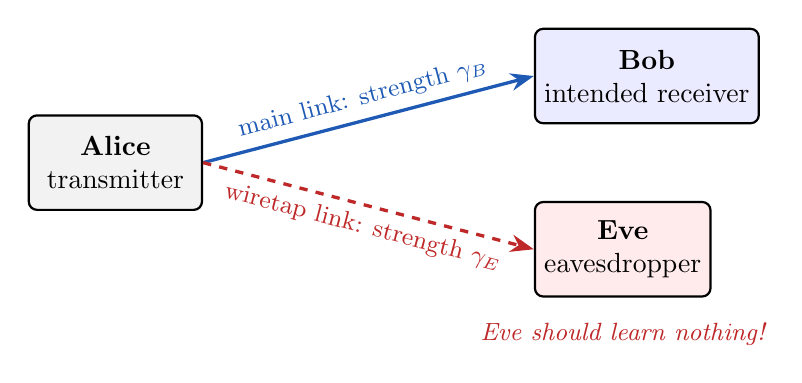
\begin{tikzpicture}[
  node distance=28mm,
  person/.style={draw, rounded corners=3pt, minimum width=22mm, minimum height=12mm,
                 align=center, thick},
  >=Stealth]
  \node[person, fill=black!5] (alice) {\textbf{Alice}\\ transmitter};
  \node[person, fill=blue!8, right=42mm of alice, yshift=11mm] (bob) {\textbf{Bob}\\ intended receiver};
  \node[person, fill=red!8,  right=42mm of alice, yshift=-11mm] (eve) {\textbf{Eve}\\ eavesdropper};
  \draw[->, very thick, bobblue] (alice.east) -- node[above, sloped, font=\small]
      {main link: strength $\gamma_B$} (bob.west);
  \draw[->, very thick, evered, dashed] (alice.east) -- node[below, sloped, font=\small]
      {wiretap link: strength $\gamma_E$} (eve.west);
  \node[below=2mm of eve, font=\small\itshape, text=evered] {Eve should learn nothing!};
\end{tikzpicture}
\end{center}

Radio signal strength is not constant. As waves bounce off walls, trees and cars, the
received strength rises and falls randomly --- this is called \textbf{fading}. You have
felt this yourself: your phone's signal bars change as you walk around a room.

So both Bob's signal strength $\gamma_B$ and Eve's signal strength $\gamma_E$ are
\textbf{random numbers}. Information theory tells us:

\begin{ideabox}[The one rule of the game]
The message stays secret only if Bob's signal is \emph{sufficiently stronger} than
Eve's. If Eve's link becomes too good relative to Bob's, secrecy fails. This failure
event is called a \textbf{secrecy outage}, and its probability is the
\textbf{Secrecy Outage Probability (SOP)}:
\[
\mathrm{SOP} \;=\; \Pr\Big[\ \gamma_B \;<\; \tau(\gamma_E)\ \Big],
\]
where $\tau(\gamma_E)$ is a \emph{threshold} that grows when Eve's signal grows.
\end{ideabox}

The entire document is one long, careful calculation of this single probability for a
specific fading model. It is organised into six tasks:

\begin{center}
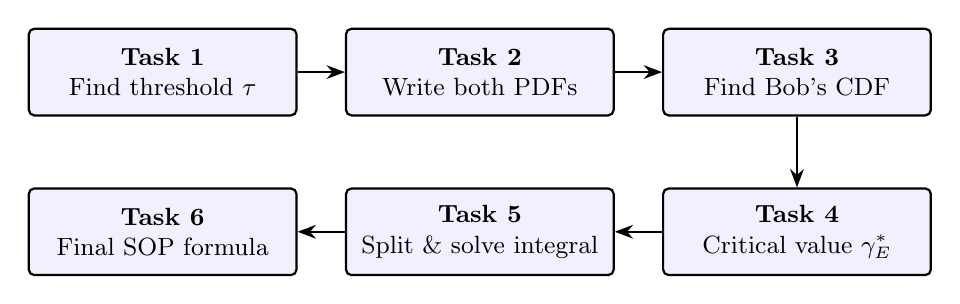
\begin{tikzpicture}[
  stp/.style={draw, rounded corners=2pt, fill=blue!6, minimum width=34mm,
               minimum height=11mm, align=center, font=\small, thick},
  >=Stealth, node distance=6mm]
  \node[stp] (t1) {\textbf{Task 1}\\ Find threshold $\tau$};
  \node[stp, right=of t1] (t2) {\textbf{Task 2}\\ Write both PDFs};
  \node[stp, right=of t2] (t3) {\textbf{Task 3}\\ Find Bob's CDF};
  \node[stp, below=9mm of t3] (t4) {\textbf{Task 4}\\ Critical value $\gamma_E^{*}$};
  \node[stp, left=of t4] (t5) {\textbf{Task 5}\\ Split \& solve integral};
  \node[stp, left=of t5] (t6) {\textbf{Task 6}\\ Final SOP formula};
  \draw[->, thick] (t1) -- (t2);
  \draw[->, thick] (t2) -- (t3);
  \draw[->, thick] (t3) -- (t4);
  \draw[->, thick] (t4) -- (t5);
  \draw[->, thick] (t5) -- (t6);
\end{tikzpicture}
\end{center}

%====================================================================
\section{The Mathematical Toolbox (Read This First)}

Two tools appear everywhere, so let us meet them once, calmly.

\subsection{Random variables, PDF, and CDF}

When a quantity is random, we describe it with two curves:

\begin{itemize}
\item The \textbf{PDF} (probability density function) $f(\gamma)$ shows \emph{where}
      the random value likes to fall. Tall parts of the curve are likely values.
      The total area under the PDF is always exactly $1$ (i.e.\ $100\%$).
\item The \textbf{CDF} (cumulative distribution function) $F(x)$ answers one question:
      \emph{``What is the chance the random value is less than $x$?''} It is simply
      the running area under the PDF from the left edge up to $x$. It starts at $0$,
      climbs, and ends at $1$.
\end{itemize}

\begin{analogybox}
Think of the heights of all students in your school. The PDF is the familiar
``most students are near average height'' curve. The CDF at $160\,$cm answers
``what fraction of students are shorter than $160\,$cm?''
\end{analogybox}

\subsection{The incomplete Beta function --- just a named area}

The model uses the function
\[
B\!\left(x;\,p,\tfrac12\right)\;=\;\int_0^x t^{\,p-1}(1-t)^{-1/2}\,\mathrm{d}t .
\]
Do not let the name scare you. It is nothing more than \textbf{the area under a
specific curve from $0$ to $x$} --- an area that appears so often in mathematics that
it earned its own name, exactly the way $\sin$, $\cos$ and $\log$ did. Your calculator
does not compute $\sin 37^\circ$ from triangles each time; it looks it up. Computers do
the same for $B(x;p,\tfrac12)$.

The document defines a compact notation used throughout:
\[
B_i^{v}(x) := B\!\left(x;\,p_v+i,\tfrac12\right),\qquad i=0,1,2,
\qquad
\Delta B_i^{v} := B_i^{v}(M_{1v}) - B_i^{v}(m_{1v}),
\]
where $v$ is either $B$ (Bob) or $E$ (Eve). So $\Delta B_i$ is just ``the area
function evaluated at the upper parameter minus at the lower parameter.''

\subsection{Three ready-made integration formulas}

Just as you memorise $\int x^2\,\mathrm{d}x = \frac{x^3}{3}$, the document proves and
then reuses three antiderivative identities:
\begin{align}
\int B_0(x)\,\mathrm{d}x &= G(x) := x\,B_0(x) - B_1(x), \tag{G}\\
\int x\,B_0(x)\,\mathrm{d}x &= H(x) := \tfrac{x^2}{2}B_0(x) - \tfrac12 B_2(x), \tag{H}\\
\int G(x)\,\mathrm{d}x &= \Phi(x) := \tfrac{x^2}{2}B_0(x) - x\,B_1(x) + \tfrac12 B_2(x). \tag{$\Phi$}
\end{align}
Each is verified the honest way: differentiate the right-hand side and check you get
back the integrand. These three formulas are the ``multiplication tables'' of the whole
derivation --- almost every later integral is solved by quoting G, H, or $\Phi$.

%====================================================================
\section{Task 1: The Threshold $\tau(\gamma_E)$}

Secrecy theory gives a rule connecting the target secrecy rate $R_s$ to the threshold
Bob must beat. For $R_s = 0.5$, the constants work out to $2^{2R_s}=2$ and the additive
constant becomes $\pi e/2$, so
\[
\boxed{\ \tau(\gamma_E) \;=\; 2\gamma_E + \frac{\pi e}{2}\ },
\qquad \frac{\pi e}{2}\approx 4.27 .
\]

\begin{analogybox}
Think of a high-jump competition where the bar keeps rising. Every unit of signal Eve
gains raises Bob's bar by \emph{two} units, and even if Eve has zero signal, Bob still
has to clear a starting bar of about $4.27$. Outage $=$ Bob fails to clear the bar.
\end{analogybox}

\begin{center}
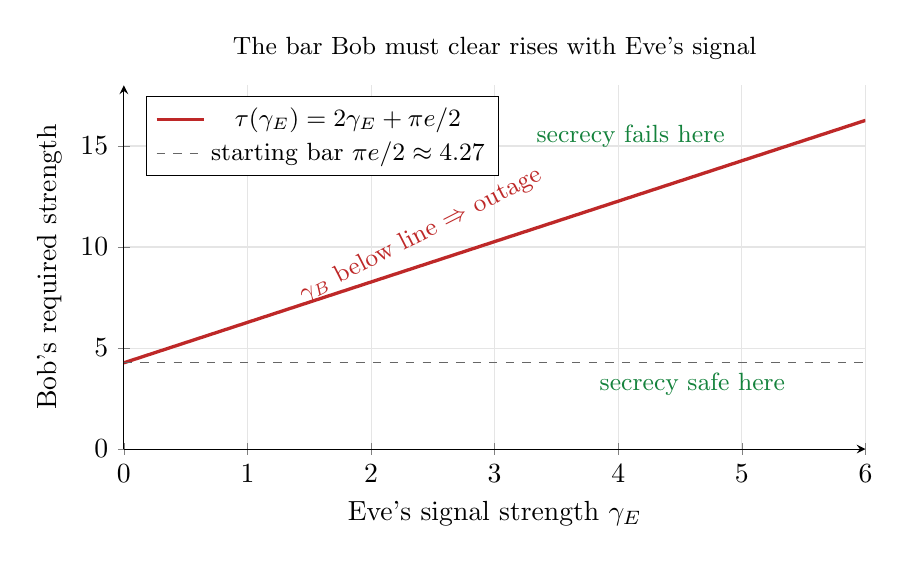
\begin{tikzpicture}
\begin{axis}[
  width=11cm, height=6.2cm,
  xlabel={Eve's signal strength $\gamma_E$},
  ylabel={Bob's required strength},
  xmin=0, xmax=6, ymin=0, ymax=18,
  axis lines=left, grid=both, grid style={black!10},
  legend pos=north west, legend style={font=\small},
  title={\small The bar Bob must clear rises with Eve's signal}]
  \addplot[very thick, evered, domain=0:6] {2*x + 4.2699};
  \addlegendentry{$\tau(\gamma_E)=2\gamma_E+\pi e/2$}
  \addplot[dashed, black!60, domain=0:6] {4.2699};
  \addlegendentry{starting bar $\pi e/2 \approx 4.27$}
  \node[font=\small, okgreen] at (axis cs:4.1,15.5) {secrecy fails here};
  \node[font=\small, okgreen] at (axis cs:4.6,3.2) {secrecy safe here};
  \node[font=\small, rotate=27, evered] at (axis cs:2.4,10.6) {$\gamma_B$ below line $\Rightarrow$ outage};
\end{axis}
\end{tikzpicture}
\end{center}

The line keeps rising ($\tau$ is strictly increasing in $\gamma_E$) --- an important
technical fact used later when we ``invert'' the relationship.

%====================================================================
\section{Task 2: The Two PDFs --- a Curve with Three Regions}

Now we need to describe how likely each signal strength is, for both Bob and Eve.
This model is unusual in two ways:

\begin{enumerate}
\item \textbf{Finite support.} The signal $\gamma$ can only lie between a smallest
      value $a_v$ and a largest value $d_v$; outside that range the probability is
      exactly zero. (Like guaranteeing every student's height is between $140$ and
      $190$ cm.)
\item \textbf{Three pieces.} Inside the support, the PDF is built from three regions:
      a \emph{rising} part, a perfectly \emph{flat} plateau, and a \emph{falling} part.
\end{enumerate}

The four breakpoints come from the model parameters:
\[
a_v=\gamma_{ov} m_{1v} m_{2v},\quad
b_v=\gamma_{ov} m_{2v} M_{1v},\quad
c_v=\gamma_{ov} m_{1v} M_{2v},\quad
d_v=\gamma_{ov} M_{1v} M_{2v},
\]
with the required ordering $a_v < b_v \le c_v < d_v$. The PDF is
\[
f_{\gamma_v}(\gamma)=
\begin{cases}
K_v\big[B_0^{v}\!\big(\tfrac{\gamma}{\gamma_{ov}m_{2v}}\big)-B_0^{v}(m_{1v})\big], & a_v\le\gamma<b_v \quad\text{(rising)},\\[1.5mm]
K_v\big[B_0^{v}(M_{1v})-B_0^{v}(m_{1v})\big], & b_v\le\gamma<c_v \quad\text{(flat)},\\[1.5mm]
K_v\big[B_0^{v}(M_{1v})-B_0^{v}\!\big(\tfrac{\gamma}{\gamma_{ov}M_{2v}}\big)\big], & c_v\le\gamma\le d_v \quad\text{(falling)},
\end{cases}
\]
and $0$ everywhere else.

\begin{center}
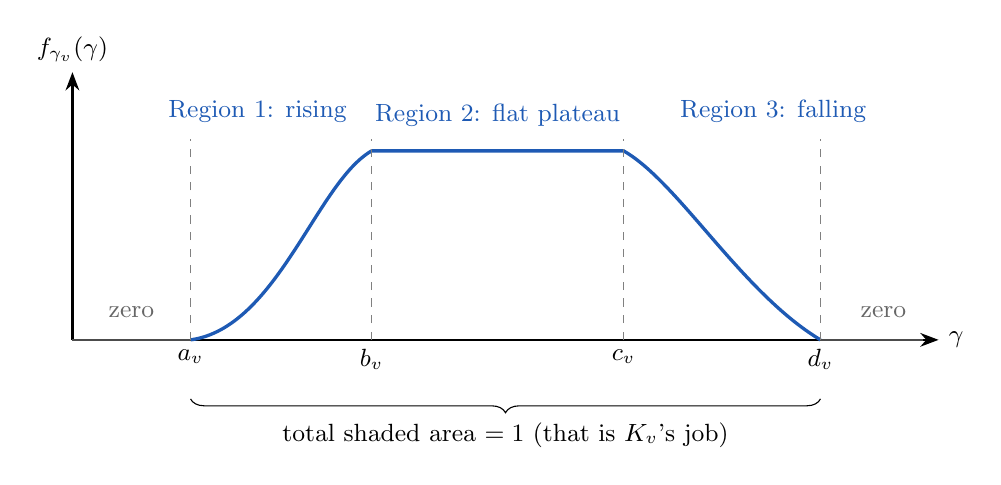
\begin{tikzpicture}[>=Stealth]
% stylised three-region PDF
\draw[->, thick] (0,0) -- (11,0) node[right, font=\small] {$\gamma$};
\draw[->, thick] (0,0) -- (0,3.4) node[above, font=\small] {$f_{\gamma_v}(\gamma)$};
% region 1 rising (smooth curve), region 2 flat, region 3 falling
\draw[very thick, bobblue]
   (1.5,0) .. controls (2.6,0.15) and (3.1,2.0) .. (3.8,2.4)
   -- (7.0,2.4)
   .. controls (7.7,2.0) and (8.5,0.6) .. (9.5,0);
\draw[thick, black!70] (0,0) -- (1.5,0);
\draw[thick, black!70] (9.5,0) -- (10.8,0);
% breakpoints
\foreach \x/\lab in {1.5/$a_v$, 3.8/$b_v$, 7.0/$c_v$, 9.5/$d_v$}{
  \draw[dashed, black!50] (\x,0) -- (\x,2.55);
  \node[below, font=\small] at (\x,0) {\lab};
}
\node[font=\small, bobblue] at (2.35,2.9) {Region 1: rising};
\node[font=\small, bobblue] at (5.4,2.85) {Region 2: flat plateau};
\node[font=\small, bobblue] at (8.9,2.9) {Region 3: falling};
\node[font=\small, black!60] at (0.75,0.35) {zero};
\node[font=\small, black!60] at (10.3,0.35) {zero};
\draw[decorate, decoration={brace, mirror, amplitude=5pt}] (1.5,-0.75) -- (9.5,-0.75)
  node[midway, below=5pt, font=\small] {total shaded area $=1$ (that is $K_v$'s job)};
\end{tikzpicture}
\end{center}

\subsection{The normalisation constant $K_v$}

$K_v$ is a scaling knob. The three-region shape above must have total area exactly
$1$; $K_v$ stretches or squashes the curve vertically until it does. The model
specifies $K_v$ by a finite double-sum formula (a sum over $i=1,2,3$ and a binomial
expansion --- messy to look at, but just arithmetic).

The document then does something clever: it \emph{independently} integrates the three
regions using identity (G). When the three region-areas are added, the $\Delta B_0$
terms \textbf{cancel in pairs} (``telescope''), leaving a beautifully short condition:
\[
\boxed{\ K_v\,\gamma_{ov}\,(M_{2v}-m_{2v})\,\Delta B_1^{v} \;=\; 1\ }.
\]

\begin{ideabox}[Why two formulas for the same $K_v$?]
Having two independent routes to $K_v$ --- the model's double sum and the telescoped
identity --- gives a built-in \textbf{self-check}: if a computer program produces a
$K_v$ that violates the boxed identity, something is wrong. The authors report the
check passes to $10^{-12}$ accuracy. This is like solving a maths problem two
different ways and getting the same answer --- strong evidence you didn't slip.
\end{ideabox}

%====================================================================
\section{Task 3: Bob's CDF --- the Running Total}

The CDF is the running area under the PDF. Since the PDF has three pieces, so does the
CDF, and the pieces must be \textbf{glued continuously} (no sudden jumps --- a running
total can never jump).

\begin{itemize}
\item \textbf{Region 1} ($a_B\le x<b_B$): integrate the rising piece using identity
      (G). The CDF here is a combination of $G_B$ evaluated at a scaled argument and a
      simple linear term.
\item \textbf{Region 2} ($b_B\le x<c_B$): the PDF is flat, so the running area grows
      \emph{linearly}: $F(x) = F(b_B) + K_B\,\Delta B_0^{B}\,(x-b_B)$. (Constant
      speed $\Rightarrow$ distance grows in a straight line.)
\item \textbf{Region 3} ($c_B\le x\le d_B$): integrate the falling piece, again via
      (G), starting from the accumulated value $F(c_B)$.
\end{itemize}

\begin{center}
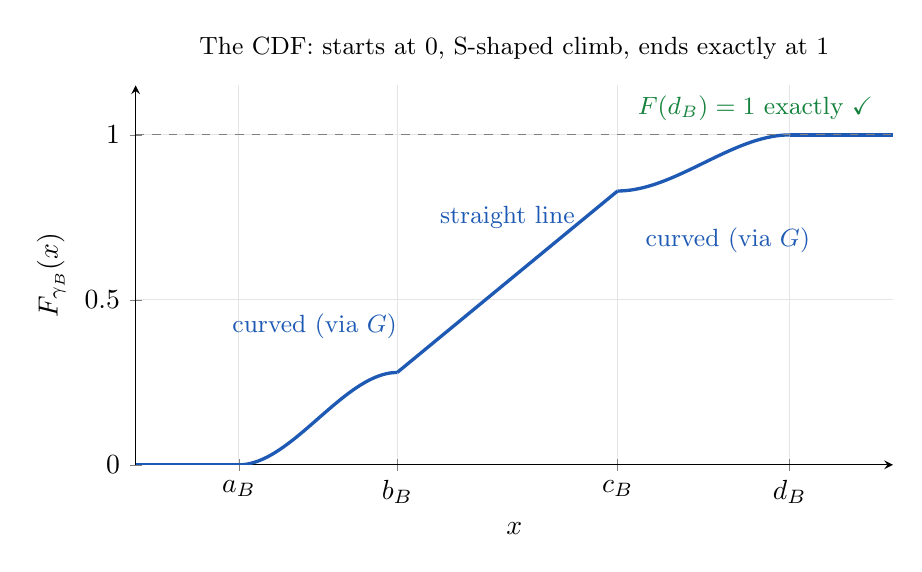
\begin{tikzpicture}
\begin{axis}[
  width=11.2cm, height=6.4cm,
  xlabel={$x$}, ylabel={$F_{\gamma_B}(x)$},
  xmin=0, xmax=11, ymin=0, ymax=1.15,
  axis lines=left, grid=both, grid style={black!10},
  xtick={1.5,3.8,7.0,9.5},
  xticklabels={$a_B$,$b_B$,$c_B$,$d_B$},
  ytick={0,0.5,1},
  title={\small The CDF: starts at 0, S-shaped climb, ends exactly at 1}]
  % piecewise smooth-ish CDF: slow start, linear middle, slow finish
  \addplot[very thick, bobblue, domain=0:1.5] {0};
  \addplot[very thick, bobblue, domain=1.5:3.8, samples=40]
     {0.28*((x-1.5)/2.3)^2*(3-2*(x-1.5)/2.3)};
  \addplot[very thick, bobblue, domain=3.8:7.0] {0.28 + 0.55*(x-3.8)/3.2};
  \addplot[very thick, bobblue, domain=7.0:9.5, samples=40]
     {0.83 + 0.17*(1-(1-(x-7)/2.5)^2*(3-2*(1-(x-7)/2.5))/1)};
  \addplot[very thick, bobblue, domain=9.5:11] {1};
  \addplot[dashed, black!50, domain=0:11] {1};
  \node[font=\small, bobblue] at (axis cs:2.6,0.42) {curved (via $G$)};
  \node[font=\small, bobblue] at (axis cs:5.4,0.75) {straight line};
  \node[font=\small, bobblue] at (axis cs:8.6,0.68) {curved (via $G$)};
  \node[font=\small, okgreen] at (axis cs:9.0,1.08) {$F(d_B)=1$ exactly \checkmark};
\end{axis}
\end{tikzpicture}
\end{center}

\textbf{The consistency check.} Plug $x=d_B$ into the Region-3 formula. Using the
boxed $K$-identity from Task 2, everything collapses to exactly $1$. This is the
mathematics confirming ``the total probability is $100\%$'' --- the running total
reaches the top of the tank precisely when the support ends.

\paragraph{A compact form for later.} On every region the CDF can be written in one
template:
\[
F_{\gamma_B}(x) = c_r + \lambda_r x + \mu_r\, G_B\!\left(\frac{x}{w_r}\right),
\]
i.e.\ ``a constant, plus a straight-line part, plus a $G$-shaped part.'' In Region 2
the $G$-part switches off ($\mu_2=0$). This template is what makes Task 5 manageable.
Eve's CDF is the identical construction with $E$ subscripts.

%====================================================================
\section{Task 4: The Critical Value $\gamma_E^{*}$ --- When Eve Is Unbeatable}

Bob's signal can \emph{never} exceed his maximum $d_B$ (finite support!). So if Eve is
strong enough that the bar $\tau(\gamma_E)$ is set above $d_B$, Bob cannot possibly
clear it --- outage is \textbf{guaranteed}, no calculation needed. The switch-over
point solves $2\gamma_E^{*} + \pi e/2 = d_B$:
\[
\boxed{\ \gamma_E^{*} \;=\; \frac{\gamma_{oB} M_{1B} M_{2B}}{2} - \frac{\pi e}{4}\ }.
\]

\begin{center}
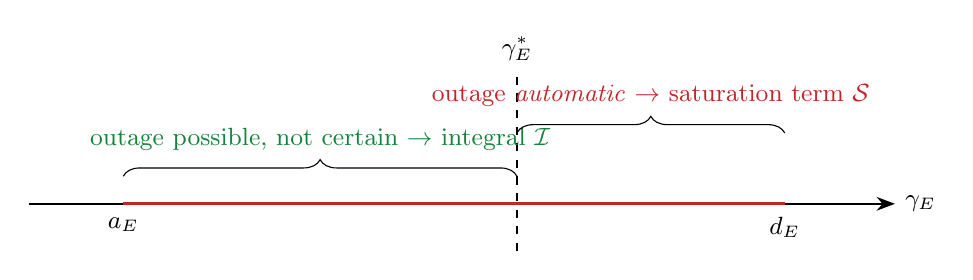
\begin{tikzpicture}[>=Stealth]
\draw[->, thick] (0,0) -- (11,0) node[right, font=\small] {$\gamma_E$};
% Eve's support
\draw[very thick, evered] (1.2,0) -- (9.6,0);
\node[below, font=\small] at (1.2,-0.05) {$a_E$};
\node[below, font=\small] at (9.6,-0.05) {$d_E$};
\draw[dashed, thick] (6.2,-0.6) -- (6.2,1.7);
\node[above, font=\small] at (6.2,1.7) {$\gamma_E^{*}$};
\draw[decorate, decoration={brace, amplitude=6pt}] (1.2,0.35) -- (6.2,0.35)
  node[midway, above=6pt, font=\small, okgreen] {outage possible, not certain $\to$ integral $\mathcal I$};
\draw[decorate, decoration={brace, amplitude=6pt}] (6.2,0.9) -- (9.6,0.9)
  node[midway, above=6pt, font=\small, evered] {outage \emph{automatic} $\to$ saturation term $\mathcal S$};
\end{tikzpicture}
\end{center}

Two corner cases follow immediately:
if $\gamma_E^{*}\le a_E$ (or is negative), the ``automatic outage'' zone covers
Eve's \emph{entire} support, so $\mathrm{SOP}=1$; if $\gamma_E^{*}\ge d_E$, the
automatic zone is empty and $\mathcal S = 0$.

%====================================================================
\section{Task 5: Splitting and Solving the SOP Integral}

Using the picture above, the SOP splits into two parts:
\[
\mathrm{SOP}
=\underbrace{\int_{0}^{\gamma_E^{*}} F_{\gamma_B}\!\big(2\gamma+\tfrac{\pi e}{2}\big)\, f_{\gamma_E}(\gamma)\,\mathrm{d}\gamma}_{\mathcal I \ \text{(fair contest)}}
\;+\;
\underbrace{1-F_{\gamma_E}(\gamma_E^{*})}_{\mathcal S \ \text{(rigged: Eve too strong)}} .
\]

\begin{analogybox}
Chance of losing a game $=$ (chance of losing a fair round) $+$ (chance the round was
rigged from the start). $\mathcal S$ is the rigged part: it needs no integral at all,
just Eve's CDF evaluated once at $\gamma_E^{*}$ --- fully closed form thanks to Task 3.
\end{analogybox}

\subsection{Why the integral must be chopped up}

Inside $\mathcal I$, two piecewise functions are multiplied: Bob's 3-region CDF
(evaluated at the moving point $2\gamma + \pi e/2$) and Eve's 3-region PDF. Each
function changes its formula at its own breakpoints. So the integration range
$[\mathcal L,\mathcal U]$ is partitioned at every point where \emph{either} formula
switches --- at most $4$ interior cut points, giving at most $N\le 5$ sub-intervals.
On each sub-interval, exactly one (Bob-region $r$, Eve-region $s$) pair is active.

\begin{center}
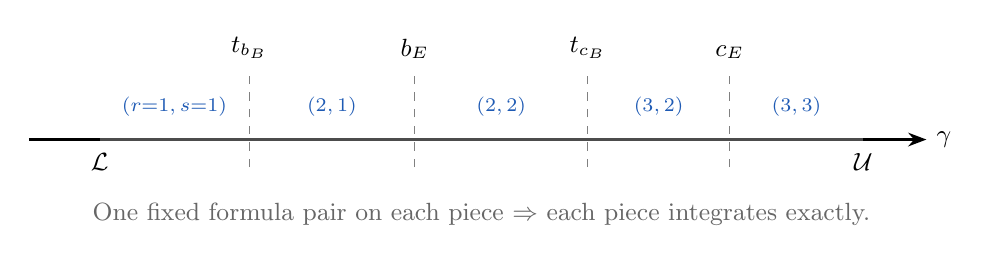
\begin{tikzpicture}[>=Stealth]
\draw[->, thick] (0,0) -- (11.4,0) node[right, font=\small] {$\gamma$};
\draw[very thick, black!70] (0.9,0) -- (10.6,0);
\node[below, font=\small] at (0.9,-0.05) {$\mathcal L$};
\node[below, font=\small] at (10.6,-0.05) {$\mathcal U$};
\foreach \x/\lab in {2.8/$t_{b_B}$, 4.9/$b_E$, 7.1/$t_{c_B}$, 8.9/$c_E$}{
  \draw[dashed, black!50] (\x,-0.35) -- (\x,0.9);
  \node[above, font=\small] at (\x,0.9) {\lab};
}
\foreach \a/\b/\lab in {0.9/2.8/{$(r{=}1,s{=}1)$}, 2.8/4.9/{$(2,1)$}, 4.9/7.1/{$(2,2)$},
                        7.1/8.9/{$(3,2)$}, 8.9/10.6/{$(3,3)$}}{
  \node[font=\scriptsize, bobblue] at ({(\a+\b)/2},0.42) {\lab};
}
\node[font=\small, black!60] at (5.75,-0.95)
  {One fixed formula pair on each piece $\Rightarrow$ each piece integrates exactly.};
\end{tikzpicture}
\end{center}

(The points $t_{b_B}, t_{c_B}$ are Bob's breakpoints ``pulled back'' through the
threshold: $t_x = (x-\pi e/2)/2$, using the fact that $\tau$ is strictly increasing.)

\subsection{Four term types on each piece}

On a sub-interval, multiply out the two brackets
\[
\underbrace{\Big[\tilde A_r+\tilde B_r\gamma+\mu_r\, G_B(\cdot)\Big]}_{\text{Bob's CDF template}}
\times
\underbrace{\Big[q_s+\nu_s\, B_0^{E}(\cdot)\Big]}_{\text{Eve's PDF template}}
\]
and exactly four kinds of terms appear:

\begin{center}
\small
\begin{tabular}{clll}
\toprule
Type & What it looks like & How it is solved & Difficulty\\
\midrule
T1 & $(\text{const}+\text{linear})\times\text{const}$ & school algebra & trivial\\
T2 & $(\text{const}+\text{linear})\times B_0^{E}$ & identities (G) and (H) & easy\\
T3 & $G_B \times \text{const}$ & identity ($\Phi$) & easy\\
T4 & $G_B \times B_0^{E}$ \ (\emph{cross term}) & series / Appell $F_1$ & the hard one\\
\bottomrule
\end{tabular}
\end{center}

\subsection{The cross term $J_{n,i}$ --- the one honest difficulty}

\begin{warnbox}
T4 multiplies \emph{Bob's} Beta function by \emph{Eve's} Beta function, each with its
own argument. For general (non-integer) shape parameters $p_B, p_E$, this product has
\textbf{no elementary antiderivative} --- and the document proves this is a genuine
mathematical fact, not a gap in the work. The exact reduction is: expand one Beta
function as a convergent power series (all arguments stay in $[0,1]$, so the series
always converges), integrate term by term, and each term becomes an Euler-type
integral expressible in \emph{Appell $F_1$ hypergeometric functions}.
\end{warnbox}

Three softening facts:
\begin{enumerate}
\item If $p_B$ (or $p_E$) is a positive whole number, the Beta function collapses to
      powers and square roots, and $J_{n,i}$ becomes a finite elementary sum.
\item $J_{n,i}$ only appears when $\mu_r \nu_s \ne 0$ --- i.e.\ when \emph{neither}
      link sits in its flat Region 2. Whenever either one is in the plateau, the cross
      term vanishes entirely. Only a handful survive.
\item Even in the worst case, $J_{n,i}$ is a smooth integral over a finite interval:
      a computer evaluates it to any precision you like.
\end{enumerate}

%====================================================================
\section{Task 6: The Final Formula}

Add everything up: for each sub-interval $j$ (with its active pair $(r_j,s_j)$), sum
the T1, T2, T3 and T4 contributions, then add the saturation term:
\[
\boxed{\ \mathrm{SOP} \;=\; \sum_{j=1}^{N}\Big[\ \text{T1}_j + \text{T2}_j + \text{T3}_j + \text{T4}_j\ \Big]
\;+\; 1 - F_{\gamma_E}(\gamma_E^{*})\ },
\qquad
\gamma_E^{*}=\frac{\gamma_{oB}M_{1B}M_{2B}}{2}-\frac{\pi e}{4}.
\]
Every symbol inside is known in closed form (via $G$, $H$, $\Phi$, the CDFs, and the
constants), except the few cross terms $J_{n,i}$, which have the exact hypergeometric
reduction described above.

The formula also passes its own sanity limits: $\gamma_E^{*}\ge d_E$ forces
$\mathcal S = 0$; $\gamma_E^{*}\le a_E$ forces $\mathrm{SOP}=1$; and if even Bob's
\emph{minimum} bar exceeds Eve's whole support ($t_{a_B}\ge d_E$), the integral
vanishes and only the saturation term remains.

%====================================================================
\section{How the Authors Checked Their Work (The Best Part)}

A derivation this long is easy to get wrong, so the authors verified it the way a
careful student verifies an exam answer --- \textbf{by solving the problem a second,
completely independent way}:

\begin{center}
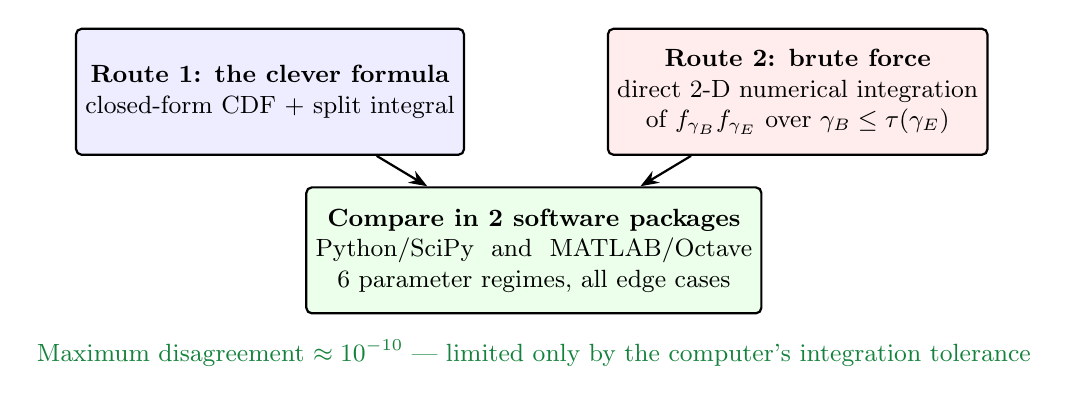
\begin{tikzpicture}[
  box/.style={draw, rounded corners=2pt, minimum width=44mm, minimum height=16mm,
              align=center, font=\small, thick},
  >=Stealth]
  \node[box, fill=blue!7] (a) {\textbf{Route 1: the clever formula}\\ closed-form CDF + split integral};
  \node[box, fill=red!7, right=18mm of a] (b) {\textbf{Route 2: brute force}\\ direct 2-D numerical integration\\ of $f_{\gamma_B} f_{\gamma_E}$ over $\gamma_B \le \tau(\gamma_E)$};
  \node[box, fill=green!8, below=12mm of $(a)!0.5!(b)$] (c)
       {\textbf{Compare in 2 software packages}\\ Python/SciPy \ and \ MATLAB/Octave\\ 6 parameter regimes, all edge cases};
  \draw[->, thick] (a) -- (c);
  \draw[->, thick] (b) -- (c);
  \node[below=2mm of c, font=\small, okgreen]
     {Maximum disagreement $\approx 10^{-10}$ --- limited only by the computer's integration tolerance};
\end{tikzpicture}
\end{center}

A sample of the reported results:

\begin{center}\small
\begin{tabular}{lccc}
\toprule
Test regime & Split formula & Brute force & $|\Delta|$\\
\midrule
Generic case & 0.5409547877 & 0.5409547880 & $2.4\times10^{-10}$\\
Weak Bob ($\mathrm{SOP}=1$ limit) & 1.0000000000 & 1.0000000000 & $1.4\times10^{-11}$\\
Strong Bob (rare outage) & 0.0000756869 & 0.0000756869 & $9.6\times10^{-15}$\\
Symmetric links & 0.7966602963 & 0.7966602962 & $1.5\times10^{-10}$\\
Nonzero saturation ($\mathcal S=0.7262$) & 0.9517435993 & 0.9517435993 & $4.4\times10^{-16}$\\
\bottomrule
\end{tabular}
\end{center}

They also confirmed: both PDFs integrate to $1$ (to $10^{-12}$); the closed-form CDF
matches a purely numerical CDF at 41 test points (to $\sim 10^{-16}$); the three
antiderivative identities survive numerical differentiation; and Python and Octave
agree to all ten printed digits. A companion program \texttt{sop\_analysis.m}
implements everything with built-in assertion checks.

%====================================================================
\section{One-Page Summary}

\begin{tcolorbox}[colback=softgray, colframe=black!40, title=\textbf{The whole document in seven sentences}]
\begin{enumerate}
\item Bob and Eve both receive a random-strength signal described by a three-piece
      (rising--flat--falling) probability curve on a finite range, built from
      incomplete Beta functions.
\item Secrecy fails when Bob's strength drops below a bar
      $\tau(\gamma_E)=2\gamma_E+\pi e/2$ that rises with Eve's strength.
\item The constant $K$ scales each curve so its total area is 1, and a telescoping
      identity pins $K$ down in one clean equation.
\item Integrating the PDF piece by piece --- and gluing at the seams --- gives Bob's
      exact three-piece CDF, which provably reaches exactly 1 at the top of the range.
\item Because Bob's strength is capped at $d_B$, Eve values above the critical point
      $\gamma_E^{*}$ make outage automatic; this contributes a closed-form
      ``saturation'' probability.
\item Below $\gamma_E^{*}$, the outage probability is an integral that chops into at
      most five pieces, each solved exactly by three reusable antiderivative
      identities --- except one stubborn cross term, which genuinely requires
      hypergeometric ($F_1$) functions unless the shape parameters are whole numbers.
\item Every formula was double-checked against brute-force numerical integration in
      two independent software systems, agreeing to about ten decimal places.
\end{enumerate}
\end{tcolorbox}

\end{document}
